\newpage
\section{Experimental Results on Simulators and Quantum Computers}
\subsection{Testing the Addition and Subtraction operations on the Aer Simulator and on a real Quantum Computer}

We will now demonstrate all of the operations of the Quantum ALU starting with addition and subtraction. Before executing any arithmetic and logic 
operation we have to initialize the Opcode register with the appropriate opcode (see Table 6.1).

Therefore, to perform an addition, the Opcode register must be initialized with the $\ket{00}$ state. For this demonstration
registers A and B are initialized with the states $\ket{11}=\ket{3}$ and $\ket{10}=\ket{2}$ respectively Listing (28):

\begin{listing}[!ht]
        \begin{minted}{python3}
            qalu.x(a[0])
            qalu.x(a[1]) # a = 11
            qalu.x(b[1]) # b = 10
        \end{minted}
        \caption{Initializing the Quantum registers A and B with the appropriate values}
        \label{ls:6_init_add}
\end{listing}

Executing the Quantum ALU circuit on an Aer simulator, the Output register arrives at the state $\ket{00000101}=\ket{5}$ which is the expected value.
In Figure (6.3) we can see this even more clearly (we omitted the five leading zeros for a clearer picture of the result):

\begin{figure}[!ht]
        \centering
        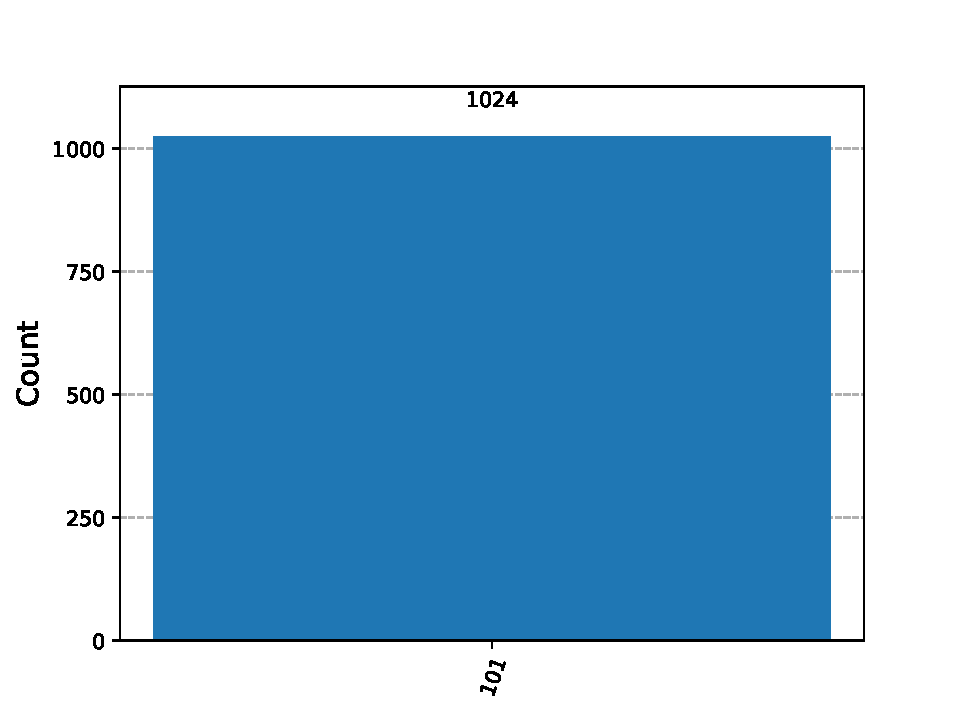
\includegraphics[scale=0.7]{images/6_Complete_System/adder_subtractor_aer_result.pdf}
        \caption{The histogram of the possible values of the Output register when the Quantum ALU performed an addition with A=3 and B=2 on the Aer Simulator}
\end{figure}

We shall now execute a subtraction operation with the same initial values for the A and B registers and submit a job to an IBM Quantum Computer
so that the circuit can be executed. We want to note that the expected output is $101_2$ which can be interpreted in many ways but because
the Adder-Subtractor implements a design where it performs signed and unsigned-mangitude addition and subtraction and because $A @> B$ the
third qubit of the output register can be omitted thus the result becomes $01_2$ or just $1$ which is the expected output. 

In Figure (6.4) we can see multiple expected output values. Although we did not use any gate that puts any qubit in superposition, Quantum Computers
are vulnerable to noise. Noise, just like in classical computers, can cause problems like flipping a single bit's state from example; a memory cell
of a Random Access Memory module. In the case of the Quantum computer, a qubit can be flipped and give erroneous results.

\begin{figure}[!ht]
        \centering
        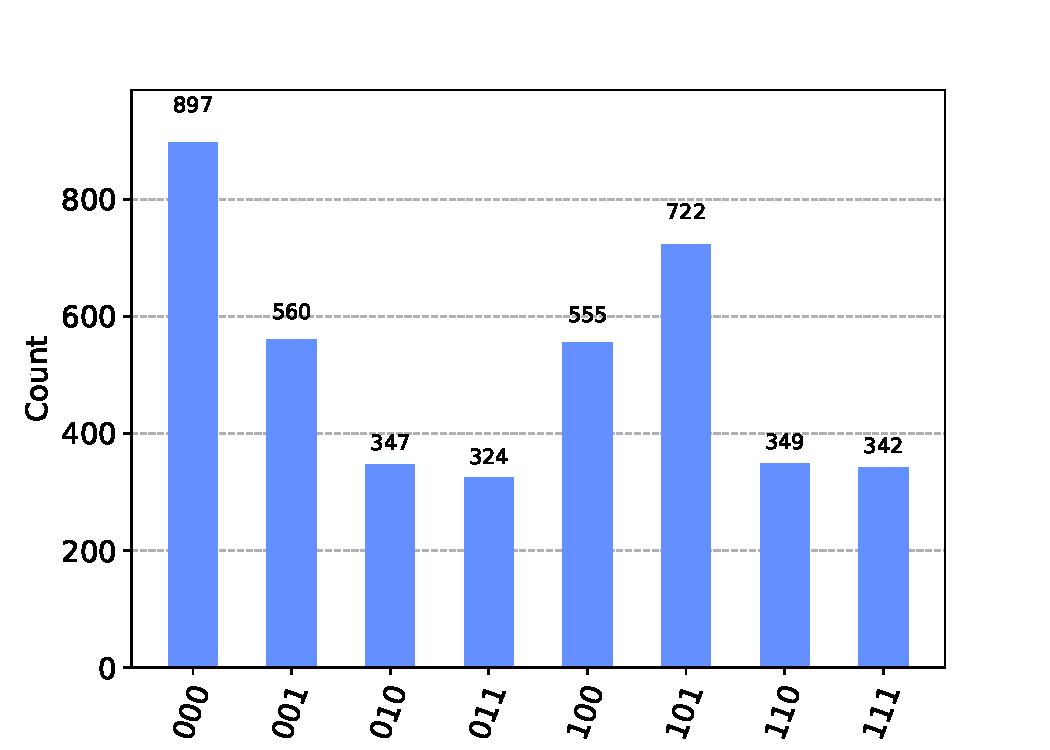
\includegraphics[scale=0.7]{images/6_Complete_System/adder_subtractor_ibmq_result.pdf}
        \caption{The histogram of the possible values of the Output register (with omitted the five leading zero'ed qubits) when the Quantum ALU performed
        an addition with A=3 and B=2 on the IBM Kyoto Quantum Computer}
\end{figure}

We can see that the expected value ($101_2$) has a probability of $17.64\%$ to be output'ed by the circuit.

\newpage
\subsection{Testing the Multiplication operation on the Aer Simulator and on a real Quantum Computer}
We shall demonstrate the multiplication operation with another pair of inputs. This time we shall initialize both A and B with the same value. We
arbitrarily chose $10_2$ or $2_{10}$.

Before anything else, we initialize the Opcode register with the appropriate opcode ($\ket{10}$) and then initialize the A and B registers.

\begin{listing}[!ht]
    \centering
    \begin{minted}{python3}
        qalu.x(op[1]) # op = 10
        qalu.x(a[1])
        qalu.x(b[1])
    \end{minted}
    \caption{The initialization of the Opcode, A and B Quantum registers to perform the multiplication operation}
\end{listing}

The result from the Aer simulator (see Figure (6.5))is what we expected. The result output only shows the qubits 0, 4, 6 and 7.

\begin{figure}[!ht]
    \centering
    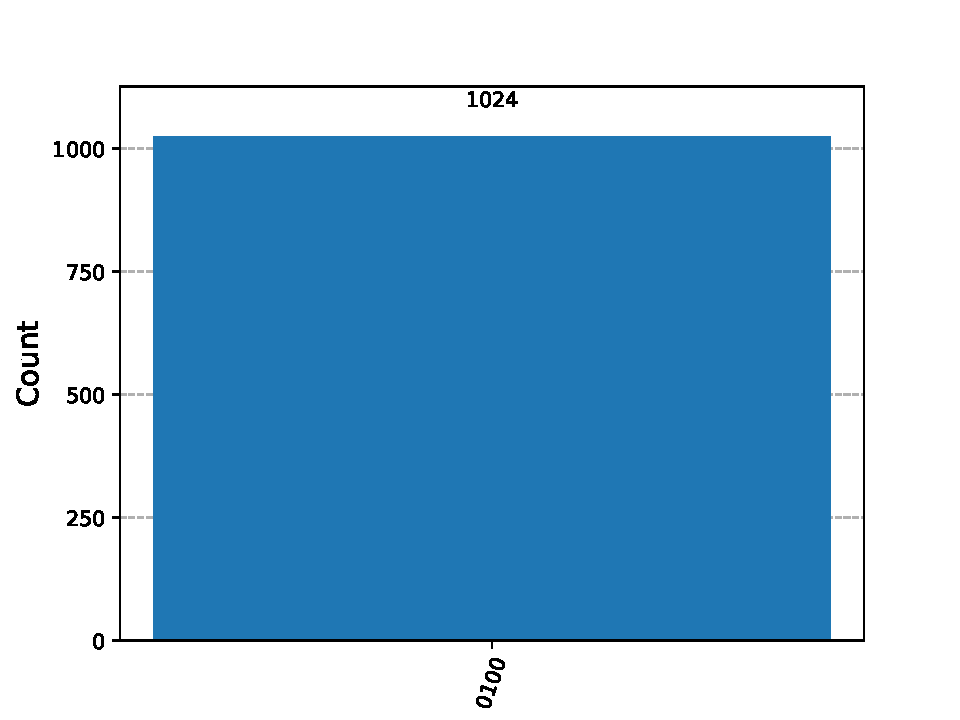
\includegraphics[scale=0.7]{images/6_Complete_System/multiplier_aer_result.pdf}
    \caption{The histogram of the possible values of the Output register when the Quantum ALU performed a multiplication with A=B=2 on the Aer Simulator}
\end{figure}

Executing the same operation on a Quantum computer yields again the same behavior. We get counts of possible outputs instead of a definite answer (see Figure (6.6)).

\begin{figure}[!ht]
        \centering
        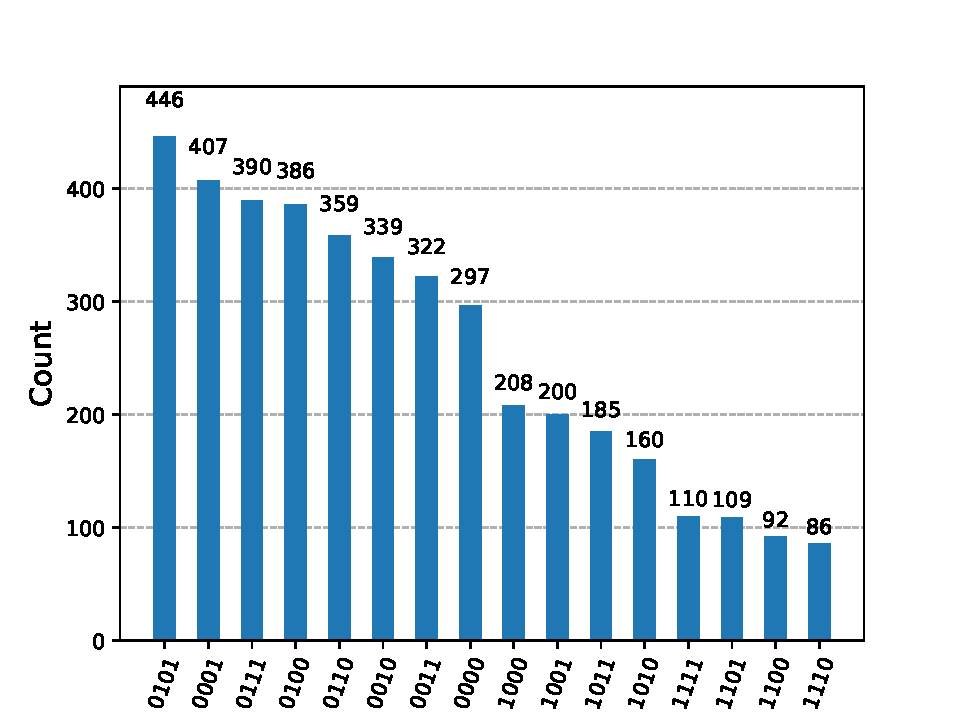
\includegraphics[scale=0.7]{images/6_Complete_System/multiplier_ibmq_result.pdf}
        \caption{The histogram of the possible values of the Output register when the Quantum ALU performed a multiplication with A=B=2 on the IBM Osaka QUantum Computer}
\end{figure}

We note that the expected output ($0100_2=4_{10}$) has a $9.42\%$ probability.

Lastly, we executed the NKO Comparator with the two two-qubit registers inputs A and B to be again $3$ and $2$ respectively and we only measured the two qubits
of the status Quantum register. The execution of the Quantum circuit happened on the IBM Osaka Quantum Computer too. We will again contrast the real-hardware result with the
simulation results.

\begin{figure}[!ht]
    \centering
    \begin{subfigure}{0.5\textwidth}
        \centering
        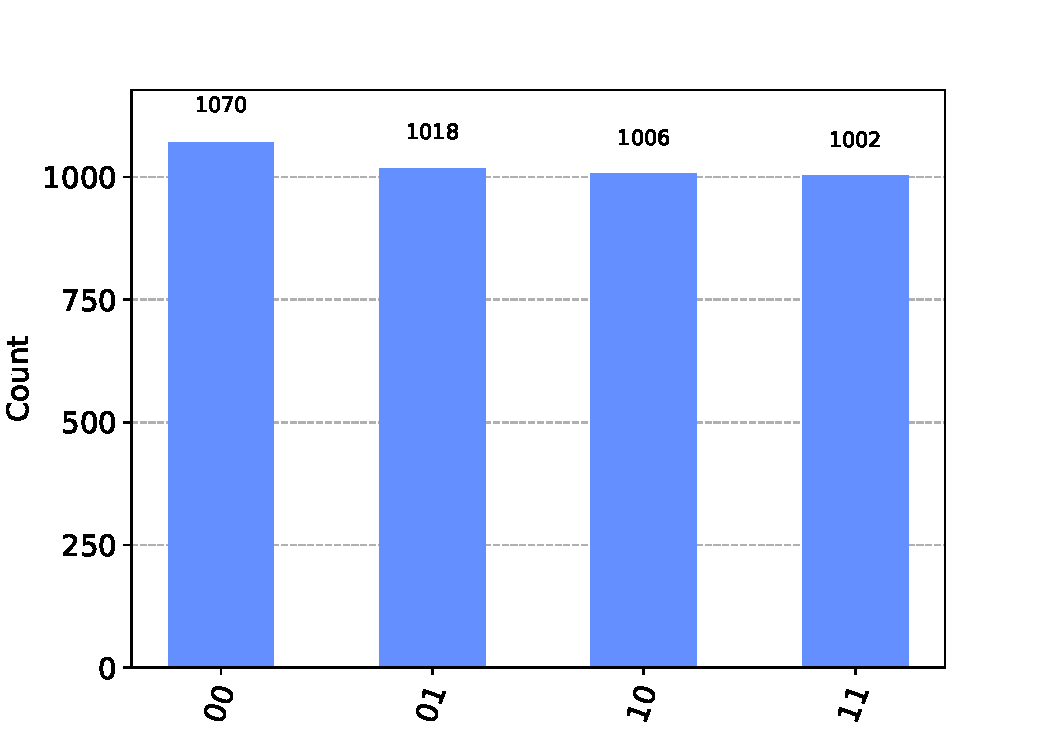
\includegraphics[scale=0.4]{images/6_Complete_System/nko_cmp_ibmq_result.pdf}
        \caption{}    
    \end{subfigure}
    \begin{subfigure}{0.5\textwidth}
        \centering
        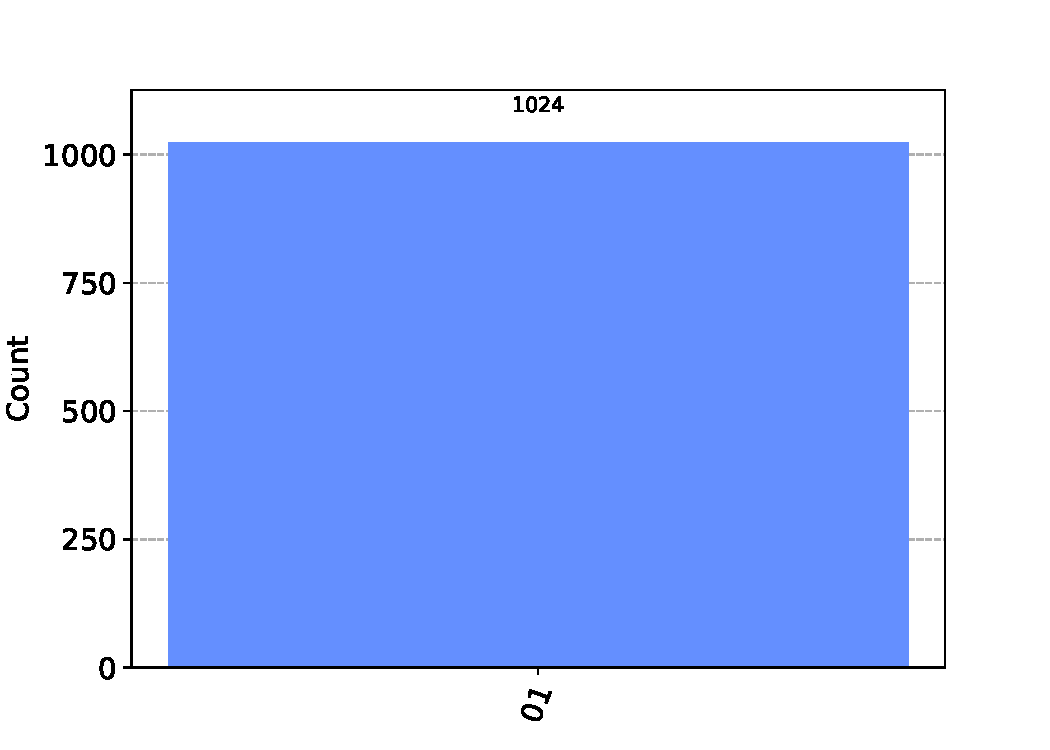
\includegraphics[scale=0.4]{images/6_Complete_System/nko_cmp_aer_result.pdf}
        \caption{}
    \end{subfigure}
    \caption{The results of the comparison operation executed on the IBM Osaka (a) and on the Aer Simulator (b)}
\end{figure}

The same story applies here, where the expected value, output'ed by the Aer Simulator, $10$ which means \say{$A\neq B\text{ and }A \geq B$}, is not the most probable output when executed
4096 times on the Quantum computer. We again compiled a table containing the probability of each output based on how many times the output occured while executing.

\begin{table}[!ht]
    \centering
    \begin{tabular}{c|c|c}
        Output Bit Sequence & Count & Probabilty ($\frac{\text{Count}}{4096}$) \\
        \hline
        $00$ & $1070$ & $26.123\%$ \\
        $01$ & $1018$ & $24.854\%$ \\
        $10$ & $1006$ & $24.561\%$ \\
        $11$ & $1002$ & $24.463\%$ \\
    \end{tabular}
    \caption{The result of probabilities of each output value of the execution of the comparison operation on the IBM Osaka}
\end{table}

We can see that each output has relatively close probability of output meaning that the Quantum computer does not give us a reliable output.